\section{Аналитическая часть}
 
Трансляция машинных кодов решает задачу запуска программ собранных под иную, по отношению к запускающей машине, архитектуру. При динамической трансляции существуют следующие проблемы:

\begin{itemize}[leftmargin=1.6\parindent]
	\item[---] выделение регистров;
	\item[---] поддержка самоизменяемого кода;
	\item[---] корректная трансляция;
	\item[---] быстрая трансляция;
	\item[---] сохранение скорости выполения кода.
\end{itemize}

Последние два пункта при динамической трансляции представляют собой смежные проблемы. Действительно, если применить все возможные оптимизации оптимизирующего компилятора LLVM к блоку трансляции этот блок будет выполнятся на высокой скорости. Однако проходы оптимизации займут большое время, что в итоге приведет к замедлению выполнения кода, нахождение этого баланса и является главной проблемой динамической трансляции. 

\subsection{Существующие решения}

В данном разделе рассматриваются методы трансляции используемые в QEMU, box64 и FEX. QEMU поддерживает эмуляцию как пользовательского режима, так и системы. box64 и FEX являются эмуляторами пользовательского режима, то есть в отличие от QEMU box64 и FEX не могут эмулировать полную систему (то есть на них нельзя, например, запустить Windows), однако можно запускать linux-приложения собранные под x86\_64.

\subsection{Трансляция}

Все рассматриваемые проекты поддерживают динамическую трансляцию для архитектуры ARM. Два из них --- QEMU и FEX --- поддерживают промежуточное представление. FEX поддерживает плохо оптимизированную трансляцию в x86 (в основном для отладки) и оптимизированную трасляцию в ARM. box64 включает в себя эмулятор, написанный на C который можно воспринимать как интерпретатор, используемый при запуске на любой архитектуре кроме ARM.

В box64 не используется промежуточное представление, таким образом при динамической рекомпиляции поддерживаемые инструкции, при помощи макросов C, транслируются в инструкции ARM. \cite{box64_letter}

Каждый блок транслируется в 4 прохода:
\begin{itemize}[leftmargin=1.6\parindent]
	\item[---] Первый проход считает все количество транслируемых x86 инструкций. Для каждой инструкции выделяется память.
	\item[---] На втором проходе обрабатываются все инструкции ветвления, проверяется где находится адрес: в этом же блоке или в каком-либо другом. В случае если адрес находится в другом блоке его необходимо связать с текущим. Также рассчитываются флаги, не нужные флаги предлагается не рассчитывать, так как инструкция может использовать/выставлять не все флаги.
	\item[---] На третьем проходе считается количество необходимых ARM инструкций в блоке.
	\item[---] На четвертом проходе генерируются необходимые инструкции.
\end{itemize}

После генерации блока он записывается в таблицу сгенерированных блоков, в которой также содержится отображение эмулированных адресов в физические. \cite{box64_wide}

В QEMU в качестве промежуточного представления используются «TCG ops», по организации похожие на инструкции архитектур RISC, эти операции сначала оптимизируются, а затем выполняются на хосте, таким образом проще портировать TCG на разные платформы. Операции поддерживаются над 32 и 64 битными целыми числами, указатели определены как псевдоним над соответствующим целым числом. \cite{qemu_readme}

Пример операции TCG представлен на листинге \ref{code:tcg}:
\begin{Verbatim}

\end{Verbatim}
\begin{code}
	\captionof{listing}{Пример операции TCG}
	\label{code:tcg}
	\begin{minted}
		[
		frame=single,
		framerule=0.5pt,
		framesep=20pt,
		fontsize=\small,
		tabsize=4,
		linenos,
		numbersep=5pt,
		xleftmargin=10pt,
		]
		{text}
add_i32 t0, t1, t2  (t0 <- t1 + t2)
	\end{minted}
\end{code}

В FEX реализованы инструкции x86, x86-64, x87, mmx, sse1, sse2, sse3, ssse3 и bmi. 

Трансляция происходит в 4 этапа:

\begin{itemize}[leftmargin=1.6\parindent]
	\item[---] Frontend: Декодирование инструкций, при декодировании также определяются границы блоков трансляции и функций.
	\item[---] OpDispatcher: Перевод инструкций во внутренние (SSA IR, IR.json) инструкции.
	\item[---] IR/Passes: Оптимизация внутренних инструкций.
	\item[---] JIT: Трансляция внутренних инструкций.
\end{itemize}

x86 инструкции декодируются в более простые для обработки, например инструкция add имеет большое количество разных опкодов, хотя по своей сути там меняются размеры и типы операндов, а не сама операция. Тогда операции add, представленные на листинге \ref{code:decode}, попадают в одну категорию.

\begin{code}
	\captionof{listing}{Пример декодирования инструкций в FEX}
	\label{code:decode}
	\begin{minted}
		[
		frame=single,
		framerule=0.5pt,
		framesep=20pt,
		fontsize=\small,
		tabsize=4,
		linenos,
		numbersep=5pt,
		xleftmargin=10pt,
		]
		{text}
00 C0: add al, al
04 01: add al, 0x1
	\end{minted}
\end{code}

Затем в качестве промежуточного представления используются СЕП инструкции напоминающие ARM. Использование СЕП облегчает оптимизацию кода, например, при устранении бессмысленных присвоений, которые показаны в листинге \ref{code:why_assign}:
\begin{code}
	\captionof{listing}{Пример лишнего присваивания}
	\label{code:why_assign}
	\begin{minted}
		[
		frame=single,
		framerule=0.5pt,
		framesep=20pt,
		fontsize=\small,
		tabsize=4,
		linenos,
		numbersep=5pt,
		xleftmargin=10pt,
		]
		{text}
y := 1
y := 2
x := y
	\end{minted}
\end{code}

Не сложно понять, что первое присвоение переменной не нужно, однако для транслятора это далеко не так очевидно. Пример использования СЕП на листинге \ref{code:SSA}:
\begin{code}
	\captionof{listing}{Использование СЕП для определения бессмысленных присвоений}
	\label{code:SSA}
	\begin{minted}
		[
		frame=single,
		framerule=0.5pt,
		framesep=20pt,
		fontsize=\small,
		tabsize=4,
		linenos,
		numbersep=5pt,
		xleftmargin=10pt,
		]
		{text}
y1 := 1
y2 := 2
x1 := y2
	\end{minted}
\end{code}

СЕП решает следующие задачи:
\begin{itemize}[leftmargin=1.6\parindent]
	\item[---] свёртка констант;
	\item[---] удаление мёртвого кода;
	\item[---] частичное устранение избыточности;
	\item[---] снижение стоимости операций;
	\item[---] распределение регистров.
\end{itemize}

После трансляции в IR количество инструкций больше изначального в 10-30 раз. 32-х битные инструкции расширяются до 64 бит.

\subsection{Использование блоков трансляции}

Блоки трансляции используются в каждом из рассматриваемых трансляторов.

В QEMU как блок трансляции выделяется часть кода до момента изменения состояния процессора которое нельзя выяснить на этапе трансляции (например, некоторое ветвление). \cite{qemu_docs}

В box64, так же как и в QEMU, код разбивается на блоки трансляции, блок заканчивается когда после нее нет других инструкций (например jump, call или ret) и когда на последнюю инструкцию не ссылается какое-либо ветвление из этого блока. Исключением являются многобайтовые NOP инструкции, которые обрабатываются отдельно, а прочтение неизвестной инструкции останавливает процесс выполнения блока. \cite{box64_letter}

В FEX Frontend.cpp разбивает код на блоки трансляции. Блок так же заканчивается при потере управления, однако рассматривается ситуация когда блоки трансляции находятся в одном месте. Некоторые трансляторы заканчивают трансляцию при любой потере управления, хотя в скомпилированном коде часто встречаются конструкции похожие на листинг \ref{code:compiled}:

\begin{code}
	\captionof{listing}{Пример кода, сгенерированного компилятором}
	\label{code:compiled}
	\begin{minted}
		[
		frame=single,
		framerule=0.5pt,
		framesep=20pt,
		fontsize=\small,
		tabsize=4,
		linenos,
		numbersep=5pt,
		xleftmargin=10pt,
		]
		{text}
test eax, eax
jne .Continue
ret           <--- Можно продолжать трансляцию после 
                   безусловной потери управления
.Continue:
	\end{minted}
\end{code}

Если можно определить адрес условного перехода, то есть возможность продолжить трансляцию. \cite{fex_front}

\subsubsection{Связывание блоков трансляции}

Одной из важных отпимизаций является связывание различных блоков трансляции. Если не связывать блоки необходимо выходить из цикла выполнения кода, проходит эпилог процедуры и затем искать следующий, необходимый блок.

Например, после выполнения одного блока трансляции QEMU ищет следующий блок, для этого используется PC (эмулируемый program counter) и другая информация о статусе процессора (например регистр CS). Сначала блок ищется в кэше трансляции, если он там не найден он достается из хэш-таблицы и добавляется в кэш. Для поиска нужно выйти из цикла выполнения блока, пройти через эпилог процедуры, найти следующий блок, запустить его, пройдя через пролог процедуры. В качестве оптимизации предлагается связывать несколько блоков трансляции напрямую.

Для этого в конце блока вызывается tcg\_gen\_lookup\_and\_goto\_ptr(), он в свою очередь вызывает helper\_lookup\_tb\_ptr который ищет нужный блок и генерирует инструкцию goto\_ptr, которая либо продолжит управление в нужном блоке, либо вернется в основной цикл трансляции. Похожая оптимизация используется при ветвлении, если ветвление происходит напрямую, в пределах одной страницы QEMU выполняет поиск блока трансляции на который будет произведено ветвление, а затем сохраняет его адрес в транслированном коде. Таким образом при следующем выполнении этого блока нет необходимости в поиске следующего блока. \cite{qemu_docs}

В box64 и FEX применяется похожая идея, таким образом сильно снижается время поиска следующего блока при безусловном ветвлении, например в FEX при выполнении 500 миллионов ветвлений поиск блока выполнялся 100 миллионов раз. \cite{fex_video}

\subsection{Поддержка самомодифицирующегося кода}

Самомодифицирующийся код на x86 представляет особую проблему, так как нет механизма оповещения об изменении кода, в отличие, например, от ARM.

При запуске в режиме пользователя QEMU помечает все страницы с транслированным кодом как защищенные от записи, при попытке записи в них поднимается сигнал SEGV, допускается запись, ИНВАЛИДИРУЕТСЯ ИЛИ КАК ТО ТАК транслированная страница и связанные с ней блоки. При запуске эмуляции системы программный MMU выполняет защиту от записи. \cite{qemu_docs}

В box64 используется похожий механизм, все транслированные страницы помечаются защищенными на запись, при попытке попытке записи страница в которую произведена запись и все последующие помечаются как "грязные". Однако, они не обязательно являются невалидными, при попытке выполнения кода с такой страницы считается CRC32, полученный результат сравнивается с контрольной суммой посчитанной при создании блока, если суммы совпадают блок объявляется валидным и опять защищается от записи, иначе генерируется новый блок. \cite{box64_letter}

В FEX не реализована полноценная поддержка самомодифицирующегося кода, один автор считает что подход QEMU и box64 является единственным приемлемым по скорости и хочет использовать его. \cite{FEX_letter}

\subsection{Оптимизации}

\subsubsection{Поддержка родных библиотек}

Одним из важных механизмов, позволяющим добиться хорошей производительности, является использование родных для архитектуры библиотек. Такой подход используется в box64 и FEX. Например, в box64 в графически требовательных приложениях производительность близка к 100\%, однако в приложениях не использующие сторонние библиотеки (то есть полностью транслируемые) производительность около 50\%.

При эмуляции Quake 3 в box64 (графического приложения с большим количеством повторно используемых функций) производительность была около 85\%.

Необходимые для работы приложения библиотеки либо транслируются, либо используется родная библиотека (в таком случае производительность выше). Вызовы функций перехватываются для вызова родных функций. 

В ELF содержатся специальные символы называемые перемещениями, они используются при линковке для установки адреса необходимой функции. При вызове родной функции в качестве адреса выставляется адрес заранее подготовленного кода, он состоит из последовательности байт \texttt{CC 53 43} и следующими за ней двух указателей. Первый указатель рассматривается как указатель на оберточную функции, а второй как указатель на обертываемую (родную) функцию. Оберточной функции передается структура с состоянием процессора и указатель на вызываемую функцию, эта структура распаковывается и вызывается переданная функция. По завершению работы оберточная функции завершается через ret или retn.

Поиск необходимой функции осуществляется при помощи файлов находящихся в src/wrapped, их необходимо определять в ручную, так как названия функций не сохраняются после компиляции программы. Сигнатура функции состоит из символов, определяющих тип возвращаемого значения и типов аргументов, разделенных буквой F. Пример сигнатуры показан на рисунке \ref{fig:box64sig}.

\begin{figure}[hbtp]
	\centering
	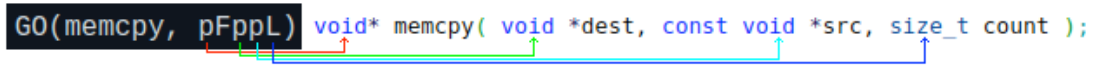
\includegraphics[width=\textwidth]{img/box64_sig.png}
	\caption{Пример сигнатуры функции memcpy}
	\label{fig:box64sig}
\end{figure}

После определения функция заносится в таблицу функций библиотеки, а затем находится при помощи разных методов. \cite{box64_deep}

В FEX так же существует поддержка родных библиотек, но, например, используется другая команда --- 0F 36, реализация сильно похожа на реализацию в box64.

\subsubsection{Оптимизации кода}

В FEX и QEMU реализованны некоторые оптимизации, свойственные оптимизирующим компиляторам, критерием выбора оптимизаций является скорость работы (так как трансляция динамическая) и эффективность.

box64 является меньшим проектом сконцентрированным на поддержке родных библиотек, поэтому в нем намного меньше оптимизаций кода.

\subsubsection{Распространение констант}

При этом проходе заменяется выражение, которое при выполнении всегда возвращает одну и ту же константу, самой этой константой. Это значение прописывается в инструкцию.

\subsubsection{Устранение мертвого кода}

Устраняется бессмысленный, не вызываемый код.
Например, на листинге \ref{code:dumb} представлена бесмысленная операция:
\begin{code}
	\captionof{listing}{Пример бессмысленной инструкции}
	\label{code:dumb}
	\begin{minted}
		[
		frame=single,
		framerule=0.5pt,
		framesep=20pt,
		fontsize=\small,
		tabsize=4,
		linenos,
		numbersep=5pt,
		xleftmargin=10pt,
		]
		{text}
  and_i32 t0, t0, $0xffffffff
	\end{minted}
\end{code}

При выполнении побитовой операции И, в которой один из аргументов равен максимально возможному для регистра числу, второй аргумент не изменит значение.

В FEX так же устраняются бессмысленные и ненужные операции.

\subsubsection{Устранение загрузок контекста}

Устраняются бесполезные загрузки контекста, например, если идет сохранение контекста, а затем сразу же его загрузка, такая загрузка выполнятся не будет. 

\subsubsection{Устранение хранения}

В QEMU подавляются неиспользуемые перемещения данных, например, в листинге \ref{code:unused} представлен пример неоптимизированного хранения:

\begin{code}
	\captionof{listing}{Пример неоптимизированных TCG инструкций}
	\label{code:unused}
	\begin{minted}
	[
	frame=single,
	framerule=0.5pt,
	framesep=20pt,
	fontsize=\small,
	tabsize=4,
	linenos,
	numbersep=5pt,
	xleftmargin=10pt,
	]
	{text}
add_i32 t0, t1, t2
add_i32 t0, t0, $1
mov_i32 t0, $1
	\end{minted}
\end{code}

После оптимизации выполнится только последняя инструкция.

В FEX устраняются бесполезные хранения, не высчитываются неиспользуемые флаги (например, те что будут перезаписаны следующей инструкцией: при операции умножения или деления используют несколько регистров и один из этих регистров будет перезаписан следующей инструкцией), если после ветвления в любом случае перезаписывается какое-либо значение --- его можно не хранить.

\subsubsection{Сжатие инструкций}

Многие x86 инструкции читают или записывают регистры подряд, можно объединять их в пары (и использовать ld2 или st1 и подобные).

Некоторые MMX операции (то есть с операндами в 64 бита) можно объединить в операции с операндами в 128 бит.

\subsubsection{Long divide removal pass}

Посоветоваться. (там шок может мне ашот расскажет)

\subsubsection{Static register allocation}

На ARM можно использовать регистровый файл, если все правильно определить регистры можно заменять store context на store registers (уточнить (может это вообще не оптимизация)).

\subsubsection{Устранение временных регистров}

В FEX, если транслируется блок, который включает в себя весь код функции, и известен используемый двоичный интерфейс, есть возможность исключить временные регистры при сохранении контекста. Также при трансляции целой функции можно убрать загрузки и сохранения в контекст посреди функции и выполнять одно сохранение в конце функции и загрузку в начале.

\subsubsection{Liveliness analysis}

В QEMU каждый регистр проверяется на используемость в определенном блоке трансляции. Если регистр не используется в блоке трансляции связанные с ним операции оптимизируются, так как значения этих регистров (и связанное с ними состояние процессора) за блок не могут измениться. Если состояние виртуального процессора меняется, такой блок не будет выполняться пока состояние процессора не будет соответствовать необходимому для блока (например, другой уровень привилегий). Например, если на x86 регистры SS, DS и SS содержат в себе 0, транслятор не будет генерировать для них смещение.

\subsubsection{Таблица методов трансляции}

\begin{table}[h]
	\begin{center}
		\label{tbl:small}
		\caption{Скорость обработки кадра (в тиках).}
			\begin{tabular}{|c|c|c|c|}
				\hline
				\bfseries Оптимизации & \bfseries QEMU & \bfseries box64 & \bfseries FEX  \\
				\hline
				Промежуточное представление & + & - & + \\ \hline
				1736*976 & 59383502 & 79846533 & 64410020 \\ \hline
				1600x1160 & 65717045 & 87026943 & 73147675 \\ \hline
				5280x3528 & 940273338 & 1156715212 & 1009131767 \\ \hline
		\end{tabular}
	\end{center}
\end{table}

\begin{comment}
кему это круто написать что это такое \cite{qemu}

\subsubsection{Сворачивание и оптимизация тривиальных выражений}

\subsubsection{Состояние процессора и блоки трансляции}


\subsubsection{Поддержка самомодифицирующегося кода}

\subsection{box64}

box64 это норм написать что такое

Одной из оптимизаций в box64, по сравнению с box86 (32-х битной версией эмулятора), является определение простых функций, такие функции не нуждаются в оберточной функции и вызываются напрямую, тем самым экономя время

\subsection{FEX}

\subsection{OpDispatcher}

Внутри FEX используется промежуточное представление, эти команды напоминают ARM64. Так как набор различных инструкций x86 слишком велик (более 1000) предлагается сначала переводить их в IR, а затем оптимизировать. На этом этапе обрабатываются особенности x86 (например MOVSB и подобные инструкции разворачиваются в циклы). OpDispatcher не выделяет регистры. 

\subsection{Трансляция IR в инструкции хоста, JIT}

При трансляции также используется кэш, для каждого потока кэш свой что приводит к избыточности, зато нет проблемы синхронизации. (это шок вообще мне надо писать про организацию кэшей в FEX?)
И еще есть LookupCache, это адреса? (вроде)
(External/FEXCore/Source/Interface/Core/LookupCache.cpp, используется в Arm64Dispatcher.cpp)

Третий уровень используется для реконструкции второго уровня в случае переполнения. Первый уровень не переполняется (разработчик так говорит).

\end{comment}

\begin{comment}
\subsection{ДАЛЬШЕ МОЖНО НЕ ЧИТАТЬ}

Список:

\begin{itemize}[leftmargin=1.6\parindent]
	\item[---] первое;
	\item[---] второе;
	\item[---] пятое;
	\item[---] десятое.
\end{itemize}

Формула:

\begin{equation}
c^2 = a^2 + b^2
\end{equation}

Ссылаемся на рисунок \ref{fig:a1}. Информация из источника \cite{golang}.

\begin{figure}[hbtp]
	\centering
	
\includegraphics[width=\textwidth]{img/golang.png}
	\caption{Пример рисунка}
	\label{fig:a1}
\end{figure}

\begin{code}
	\captionof{listing}{Пример кода}
	\label{code:1}
	\inputminted
	[
	frame=single,
	framerule=0.5pt,
	framesep=20pt,
	fontsize=\small,
	tabsize=4,
	linenos,
	numbersep=5pt,
	xleftmargin=10pt,
	]
	{text}
	{code/main.go}
\end{code}
\end{comment}

\pagebreak